%% 
%% Copyright 2007, 2008, 2009 Elsevier Ltd
%% 
%% This file is part of the 'Elsarticle Bundle'.
%% ---------------------------------------------
%% 
%% It may be distributed under the conditions of the LaTeX Project Public
%% License, either version 1.2 of this license or (at your option) any
%% later version.  The latest version of this license is in
%%    http://www.latex-project.org/lppl.txt
%% and version 1.2 or later is part of all distributions of LaTeX
%% version 1999/12/01 or later.
%% 
%% The list of all files belonging to the 'Elsarticle Bundle' is
%% given in the file `manifest.txt'.
%% 

%% Template article for Elsevier's document class `elsarticle'
%% with numbered style bibliographic references
%% SP 2008/03/01

\documentclass[preprint,12pt, a4paper]{elsarticle}

%% Use the option review to obtain double line spacing
%% \documentclass[authoryear,preprint,review,12pt]{elsarticle}

%% For including figures, graphicx.sty has been loaded in
%% elsarticle.cls. If you prefer to use the old commands
%% please give \usepackage{epsfig}

%% The amssymb package provides various useful mathematical symbols
\usepackage{amssymb}
%% The amsthm package provides extended theorem environments
%% \usepackage{amsthm}

%% The lineno packages adds line numbers. Start line numbering with
%% \begin{linenumbers}, end it with \end{linenumbers}. Or switch it on
%% for the whole article with \linenumbers.
\usepackage{lineno}

\usepackage{float}
\restylefloat{table}

\journal{SoftwareX}

\begin{document}

%%%%%%%%%%%%%%%%%%%%%%%%%%%%%%%%%%%%%%%%%%%%%%%%%%%%%%%%%%%%%%%%%%%%%%%%%%%%%%%
\begin{frontmatter}

%% Title, authors and addresses

%% use the tnoteref command within \title for footnotes;
%% use the tnotetext command for theassociated footnote;
%% use the fnref command within \author or \address for footnotes;
%% use the fntext command for theassociated footnote;
%% use the corref command within \author for corresponding author footnotes;
%% use the cortext command for theassociated footnote;
%% use the ead command for the email address,
%% and the form \ead[url] for the home page:
%% \title{Title\tnoteref{label1}}
%% \tnotetext[label1]{}
%% \author{Name\corref{cor1}\fnref{label2}}
%% \ead{email address}
%% \ead[url]{home page}
%% \fntext[label2]{}
%% \cortext[cor1]{}
%% \address{Address\fnref{label3}}
%% \fntext[label3]{}

\title{One-dimensional turbulence (ODT): computationally efficient modeling and simulation of turbulent  flows}

%% use optional labels to link authors explicitly to addresses:
%% \author[label1,label2]{}
%% \address[label1]{}
%% \address[label2]{}

%\renewcommand{\thefootnote}{\fnsymbol{footnote}}
\author{Victoria B. Stephens}
\author{David O. Lignell\corref{cor1}}

\cortext[cor1]{Corresponding author. \ead{davidlignell@byu.edu}}

\address{Chemical Engineering Department, Brigham Young University, Provo, UT 84602, USA}

\begin{abstract}
Write this last. About 100 words. 
\end{abstract}

\begin{keyword}
%% keywords here, in the form: keyword \sep keyword
turbulence \sep reacting flows \sep one-dimensional turbulence

%% PACS codes here, in the form: \PACS code \sep code

%% MSC codes here, in the form: \MSC code \sep code
%% or \MSC[2008] code \sep code (2000 is the default)

\end{keyword}

\end{frontmatter}

%%%%%%%%%%%%%%%%%%%%%%%%%%%%%%%%%%%%%%%%%%%%%%%%%%%%%%%%%%%%%%%%%%%%%%%%%%%%%%%
\section*{Code Metadata}
\label{metadata}

\begin{table}[H]
\begin{tabular}{|l|p{6.5cm}|p{6.5cm}|}
\hline
\textbf{Nr.} & \textbf{Code metadata description} & \textbf{Please fill in this column} \\
\hline
C1 & Current code version & 1.0 \\
\hline
C2 & Permanent link to code/repository used for this code version & $github.com/BYUignite/ODT$ \\
\hline
C3 & Code Ocean compute capsule & N/A\\
\hline
C4 & Legal Code License   & MIT \\
\hline
C5 & Code versioning system used & Git \\
\hline
C6 & Software code languages, tools, and services used & C++, Python 3.x, Yaml,  \\
\hline
C7 & Compilation requirements, operating environments \& dependencies & CMake 3.12+, Cantera, Git, Doxygen (optional) \\
\hline
C8 & If available Link to developer documentation/manual & N/A \\
\hline
C9 & Support email for questions & davidlignellbyu.edu \\
\hline
\end{tabular}
\caption{Code metadata (mandatory)}
\end{table}


\linenumbers

%The permanent link to code/repository or the zip archive should include the following requirements: 
%\begin{itemize}
%	\item README.txt and LICENSE.txt.
%	\item Source code in a src/ directory, not the root of the repository.
%	\item TO DO: Tag corresponding with the version of the software that is reviewed.
%	\item TO DO: Documentation in the repository in a docs/ directory, and/or READMEs, as appropriate.
%\end{itemize}

%%%%%%%%%%%%%%%%%%%%%%%%%%%%%%%%%%%%%%%%%%%%%%%%%%%%%%%%%%%%%%%%%%%%%%%%%%%%%%%
\section{Motivation and significance}
\label{sec:motivation}

Turbulent flows characterize the vast majority of fluid flows in practical engineering applications, and simulations of turbulent flows provide researchers with valuable insights into complex systems, particularly reacting turbulent flows such as combustion processes. Turbulence is a complex phemonenon that affects the full range of a flow's length and time scales. As a result, resolving the entire flow field by numerically solving the Navier-Stokes equations of fluid flow, as is done in direct numerical simulations (DNS), requires substantial computational resources. DNS is a powerful research tool, but its high computational cost makes it intractable for simulating most practical engineering flows. In order to achieve numerical solutions to practical flow problems, researchers can use alternative frameworks that model turbulence rather than resolving it directly.

Large-eddy simulations (LES) address the problem of wide-ranging length and time scales by combining  direct resolution of grid-scale quantities, as in DNS, with subgrid modeling of smaller turbulence structures. The more complex the flow, the more modeling is required; for example, a jet flame simulation might require subgrid modeling for the combustion chemistry, radiative heat transfer, or soot chemistry in addition to turbulence structures, all of which form a tightly coupled system in which each model interacts heavily with the others. While subgrid modeling makes LES more computationally affordable than DNS, it can introduce empiricism into simulations, which can lead to inaccurate results. Additionally, unresolved quantities are often parameterized in state space with empirical relationships or assumed distributions that lack universal applicability. LES is a valuable simulation tool, but its approach to turbulence modeling can introduce unwanted empiricism and make errors difficult to isolate and quantify.

The one-dimensional turbulence model (ODT) functionally reverses the LES approach, modeling large-scale turbulent advection and directly resolving small-scale flow structures, simulating the full range of length and time scales in a single dimension. Because large-scale structures are much easier to study and model than small-scale structures, ODT mitigates or sidesteps many of the subgrid modeling issues that complicate LES. Previous studies show that ODT can attain accuracy comparable to DNS at a fraction of the computational cost \cite{Lignell_2015,Abboud_2015}, making it an attractive tool for simulating turbulent flows. Because the model is one-dimensional, it is limited to homogeneous or boundary layer flows such as jets, wakes, and mixing layers; such flows, however, are extremely common in both nature and turbulence research. ODT's computational efficiency and resolution of a full range of scales make it a valuable tool that complements experimental studies and other simulation tools like DNS and LES.

%Questions to answer in this section (from SoftwareX template)
%\begin{enumerate}
%	\item What's the scientific background and motivation for this software?
%	\item Why is this important? What problems does it solve?
%	\item How has the software contributed (and/or how will it contribute in the future) to the process of scientific discovery? Cite papers using the software.
%	\item In what experimental setting might someone use this software?
%	\item What related work is there in the literature?
%	\item What algorithms, other code/software, or ideas are used? Cite them. 
%\end{enumerate}

%%%%%%%%%%%%%%%%%%%%%%%%%%%%%%%%%%%%%%%%%%%%%%%%%%%%%%%%%%%%%%%%%%%%%%%%%%%%%%%
\section{Software description}
\label{sec:description}

\subsection{Model description}
\label{sub:model_description}

The ODT model is described in detail in the literature \cite{Kerstein_1999,Kerstein_2001,Ashurst_2005,Lignell_2018,Lignell_2013}; only a brief explanation will be given here. In ODT, turbulent advection is modeled with stochastic processes called eddy events, which punctuate the solution of unsteady, one-dimensional transport equations for mass, momentum, and enthalpy. The ODT code uses a Lagrangian finite-volume formulation for diffusive advancement that includes adaptive mesh refinement \cite{Lignell_2013}. In this approach, mass remains constant inside each grid cell while cell volumes increase or decrease according to dilation. Because the ODT model is one-dimensional, it is limited to homogeneous or boundary-layer flows, such as jets, wakes, and mixing layers; these types of flows, however, are common in nature and central to turbulence research.

Eddy events occur as a Poisson process in accordance with their eddy rates, where a given eddy event of size $l$ and location $x_0$ has an eddy timescale $t$ and an associated eddy rate $1/t$. Three user-defined ODT parameters control the eddy event process: the eddy rate parameter $C$ scales the rate of occurrence of the eddies; the viscous penalty parameter $Z$ suppresses small eddies; and the large eddy suppression parameter $\beta$ constrains eddies such that they do not reach over the elapsed simulation time. 

Eddy events modify domain variables using triplet maps, as illustrated for a cylindrical domain in Figure \ref{fig:tripletmap}. For a region of eddy size $l$, the domain is copied to create three map images; the three images are then placed back to back with the middle image inverted to maintain continuity, and the composite is reapplied to the domain. This process applies to all transported variables on the domain. Applied properly, the triplet map increases scalar gradients and decreases length scales consistent with the application of turbulent eddies in real flows, conserves all quantities and their statistical moments, and maintains continuity in property profiles. Subsequent eddies in the same region will result in a cascade of scales, and eddy rates depend on eddy size and the local kinetic energy such that they follow turbulent cascade scaling laws.  

\begin{figure}
	\centering
	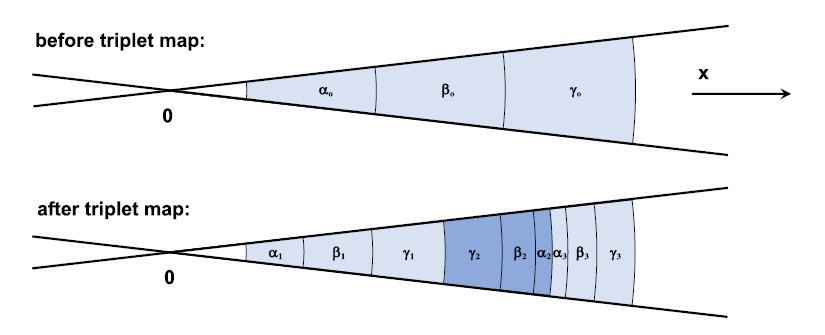
\includegraphics[width=\textwidth]{../figures/tripletmap/tripletmap.png} 
	\caption{Schematic diagram of a cylindrical triplet map, adapted from \cite{Lignell_2018}. Before the triplet map, the domain contains three grid cells of equal volume, while after the triplet map has been applied, the domain contains nine cells. The nine final cells are labeled according to the cells from which they originated and shaded to indicate that three map images were combined to create the final composite.}
	\label{fig:tripletmap}
\end{figure}

%-----------------------------------------------------------------------------------
\subsection{Software Architecture}
\label{sub:architecture}

The ODT code is a relatively self-contained C++ package. The system of nonlinear ODEs is solved using CVODE \cite{Hindmarsh_2020} and user input files are processed with YAML \cite{Beder_2008}, both of which are installed locally during the ODT build process. For reacting flow cases, chemical kinetics and transport are handled by Cantera \cite{Goodwin_2018}, which must be previously installed by the user. 

%Things to put in this section (from SoftwareX template)
%\begin{itemize}
%	\item overview of overall software architecture
%	\item optional: pictorial overview
%	\item implementation details
%\end{itemize}

%%%%%%%%%%%%%%%%%%%%%%%%%%%%%%%%%%%%%%%%%%%%%%%%%%%%%%%%%%%%%%%%%%%%%%%%%%%%%%%
\section{Example Cases}
\label{sec:examples}

%Present the major functionalities of the software. 
%\begin{itemize}
%	\item simulating turbulent flow cases, reacting or nonreacting flows
%	\item can simulate laminar flow cases too
%	\item does these things a whole lot faster than other methods do (LES, DNS especially)
%	\item testing LES subgrid modeling assumptions
%	\item simulating cases that DNS can't get to because needed simulation length is too long (i.e. late-flame phenomena)
%\end{itemize}

%Example cases:
%\begin{itemize}
%	\item From cylindrical ODT paper:
%	\begin{enumerate}
%		\item pipe flow
%		\item nonreacting round jet
%		\item round jet flame
%	\end{enumerate}
%	\item Other possible example cases:
%	\begin{itemize}
%		\item something to compare with DNS/LES results to illustrate efficiency
%		\item no sooting cases since no soot in the code
%		\item planar vs. cylindrical comparison
%	\end{itemize}
%\end{itemize} 
%
%Things to talk about with example cases:
%\begin{itemize}
%	\item compare to DNS/LES cases; computational efficiency, accuracy
%	\item how data looks before post processing, how post processing works
%\end{itemize}


%%%%%%%%%%%%%%%%%%%%%%%%%%%%%%%%%%%%%%%%%%%%%%%%%%%%%%%%%%%%%%%%%%%%%%%%%%%%%%%
\section{Impact}
\label{sec:impact}

Questions to answer in this section (from SoftwareX template)
\begin{enumerate}
	\item How can new research questions be pursued with this software?
		\begin{itemize}
			\item possibility of parametric studies (much harder with DNS/LES/RANS)
			\item study of late-flame soot and radiation interactions, soot emissions as smoke
			\item comparative radiation model studies?
		\end{itemize}
	\item How does the software improve pursuit of existing research questions?
		\begin{itemize}
			\item late-flame behavior becomes easier to study
			\item validation of LES subgrid models
			\item soot stuff, especially late in the flame (because soot moves slowly compared to gas species and therefore short simulation times like in DNS aren't enough to study it effectively)
		\end{itemize}
	\item How does the software change the daily practice of its users?
		\begin{itemize}
			\item cases take hours or days rather than weeks using supercomputer resources
			\item test cases can be run on local computers (unlike something like DNS) and as background tasks without disrupting other tasks
			\item ODT as a tool complements other approaches, can cover blind spots and be used in validation
		\end{itemize}
	\item How widespread is the software? Who uses it? (Within and outside of intended research area and/or group.)
		\begin{itemize}
			\item BYU group
			\item JCH at Sandia
			\item Chalmers group in Sweden (Marco Fistler, etc.)
			\item German university group (Heiko Schmidt, Juan Media, Marten Klein, etc.)
			\item TO DO: find other groups who have used or currently use ODT
		\end{itemize}
	\item How is the software used in commercial settings (if any)? Has it led to creation of spin-off companies?
		\begin{itemize}
			\item No commercial use (I think). 
		\end{itemize}
\end{enumerate}

%COPIED/PASTED FROM CYLINDRICAL ODT PAPER
%ODT has been applied by a number of researchers to a wide range of flows. These include homogeneous turbulence \cite{Kerstein_1999,Sun_2014}, wakes \cite{Kerstein_2000}, mixing layers \cite{Kerstein_1999,Kerstein_2001,Ashurst_2003,Ashurst_2005}, stratified flows \cite{Wunsch_2001}, Rayleigh-Benard flows \cite{Wunsch_2005}, buoyant wall flows \cite{Dreeben_2000,Shihn_2007}, and channel flows \cite{Schmidt_2009,Schmidt_2003,Lignell_2013}. Schmidt et al. \cite{Schmidt_2013} studied buoyantly-driven cloud-top entrainment with comparisons to water tank experiments. Gonzalez-Juez et al. \cite{Esteban_2013} studied reactive Rayleigh-Taylor mixing. A number of ODT simulations of turbulent jet flames have been performed \cite{Echekki_2001,Hewson_2001,Hewson_2002,Punati_2011,Lignell_2012b,Lignell_2015}. Other combustion applications include wall fires \cite{Monson_2016,Shihn_2004}, buoyant pool fires \cite{Ricks_2010,Hewson_2006,Hewson_2009}, and opposed jet flames \cite{Jozefik_2015}. Several studies used DNS to validate ODT for combustion in temporal planar jets \cite{Punati_2011,Lignell_2012b,Lignell_2015}. ODT has also been applied as a subgrid model for large eddy simulations (LES) \cite{Cao_2008,Schmidt_2003,Schmidt_2010} and in particle dynamics simulations in channel flows \cite{Schmidt_2009}, homogeneous turbulence \cite{Sun_2014}, and jets \cite{Sun_2017,Goshayeshi_2015}.

%TEXT COPIED FROM ABANDONED JOSS DRAFT

%ODT has been applied to a wide range of flows. Early applications focused on homogenous turbulence, wakes, and mixing layers (Kerstein1999,Kerstein2000,Kerstein2001). Later extension to variable-density flows and a spatial downstream coordinate system facilitated its growth and application to more complex flows, including combustion in jet flames (Echekki2001; Hewson2001; Hewson2002; Lignell2012; Punati2011; Abdelsamie2017; Lignell2017; Goshayeshi2015), counterflow flames  (Jozefik2015), wall fires (Monson2016), and sooting flames, (Lignell2015; Hewson2006; Hewson2009; Lignell2015b, Ricks2010), as well as other particle flows (Sun2017; Schmidt2009; Sun2014; Fistler2017).  ODT has also served to complement LES through subgrid modeling studies (Cao2008; Schmidt2003; Schmidt2010) and has been applied to various other flow configurations such as double-diffusive interfaces (GonzalezJuez2011), Rayleigh-Taylor mixing (GonzalezJuez2013), and stratified turbulence (Wunsch2001).  Most recently, the ODT code was extended to include cylindrical and spherical coordinate systems (Lignell2018; Klein2018; Klein2019). During this implementation, the ODT code was drastically overhauled, resulting in the SEC package presented here. Further detail on the current ODT model formulation and implementation can be found in the literature (Ashurst2005; Kerstein2001; Lignell2013; Lignell2018).

%Ongoing research involving ODT and SEC spans multiple research groups and subject areas. ODT is currently being used to investigate soot formation and destruction in ethylene jet flames via parametric modeling studies (Hewson2015; Lansinger2015b). The SEC package framework is also being used to develop the hierarchical parcel swapping model (HiPS), which models turbulence with an economical, hierarchical network that represents the fluid as individual parcels capable of switching positions within the tree (Kerstein2013; Kerstein2014). In the future, SEC may also be extended to include the linear eddy model (LEM) (Kerstein1991) and LES approaches. 

%%%%%%%%%%%%%%%%%%%%%%%%%%%%%%%%%%%%%%%%%%%%%%%%%%%%%%%%%%%%%%%%%%%%%%%%%%%%%%%
\section{Conclusion}
\label{sec:conclusion}

Write this part next to last
%Set out the conclusion of this original software publication.

%%%%%%%%%%%%%%%%%%%%%%%%%%%%%%%%%%%%%%%%%%%%%%%%%%%%%%%%%%%%%%%%%%%%%%%%%%%%%%%
\section{Conflict of Interest}
%Please select the appropriate text:
%
%Potential conflict of interest exists:
%We wish to draw the attention of the Editor to the following facts, which may be considered as potential conflicts of interest, and to significant financial contributions to this work. The nature of potential conflict of interest is described below: [Describe conflict of interest]

%No conflict of interest exists:
We wish to confirm that there are no known conflicts of interest associated with this publication and there has been no significant financial support for this work that could have influenced its outcome.

%%%%%%%%%%%%%%%%%%%%%%%%%%%%%%%%%%%%%%%%%%%%%%%%%%%%%%%%%%%%%%%%%%%%%%%%%%%%%%%
\section*{Acknowledgements}
\label{acknoledgements}

This work is supported in part by the National Science Foundation under Grant No. CBET-1403403.

%Special thanks to Alan R. Kerstein for his significant contributions to model development. Additional thanks to Heiko Schmidt, Juan Medina, and Marten Klein of Brandenburg University of Technology Cottbus-Senftenberg, Michael Oevermann and Marco Fistler of Chalmers University of Technology, and Vladimir P. Solovjov of Brigham Young University.

%%%%%%%%%%%%%%%%%%%%%%%%%%%%%%%%%%%%%%%%%%%%%%%%%%%%%%%%%%%%%%%%%%%%%%%%%%%%%%%
%% The Appendices part is started with the command \appendix;
%% appendix sections are then done as normal sections
%% \appendix

%% \section{}
%% \label{}

%%%%%%%%%%%%%%%%%%%%%%%%%%%%%%%%%%%%%%%%%%%%%%%%%%%%%%%%%%%%%%%%%%%%%%%%%%%%%%%
%% References:

\bibliographystyle{elsarticle-num} 
\bibliography{references} 

%%%%%%%%%%%%%%%%%%%%%%%%%%%%%%%%%%%%%%%%%%%%%%%%%%%%%%%%%%%%%%%%%%%%%%%%%%%%%%%
\section*{Current executable software version}
\label{software_version}

Ancillary data table required for sub version of the executable software: (x.1, x.2 etc.) kindly replace examples in right column with the correct information about your executables, and leave the left column as it is.

\begin{table}[!h]
\begin{tabular}{|l|p{6.5cm}|p{6.5cm}|}
\hline
\textbf{Nr.} & \textbf{(Executable) software metadata description} & \textbf{Please fill in this column} \\
\hline
S1 & Current software version & 2.1 \\
\hline
S2 & Permanent link to executables of this version  & For example: $https://github.com/combogenomics/$ $DuctApe/releases/tag/DuctApe-0.16.4$ \\
\hline
S3 & Legal Software License & MIT \\
\hline
S4 & Computing platforms/Operating Systems & Linux, OS X, Microsoft Windows\\
\hline
S5 & Installation requirements \& dependencies & CMake 3.12+, Cantera, Git, Doxygen (optional) \\
\hline
S6 & If available, link to user manual - if formally published include a reference to the publication in the reference list & For example: $http://mozart.github.io/documentation/$ \\
\hline
S7 & Support email for questions & davidlignell@byu.edu \\
\hline
\end{tabular}
\caption{Software metadata (optional)}
\end{table}

\end{document}
\endinput
